\section{Parte 04 – Instalacion de Oracle Data 12C} 
\begin{enumerate}[1.]
	      
	\item Ingresamos nuevamente a Administraci\'on de equipos y seleccionamos  la opci\'on de usuarios y grupos locales.\\
	\begin{center}
	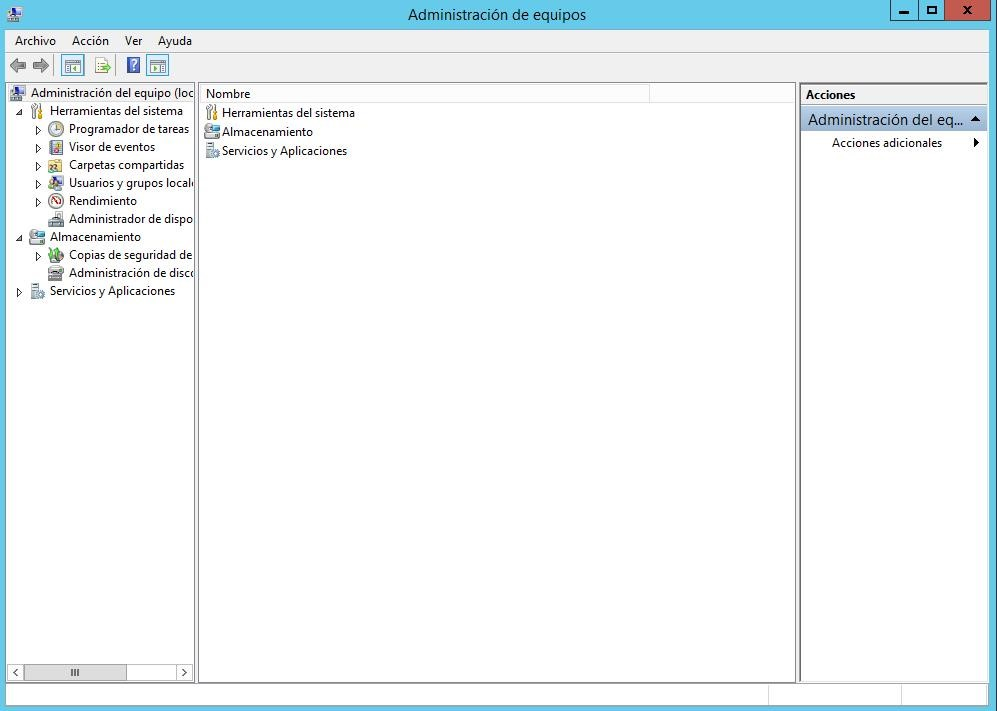
\includegraphics[width=10cm]{./Imagenes/jhordy1} 
	\end{center}
	\hfill \break	
	\hfill \break
	\hfill \break
	\hfill \break
	\begin{center}
	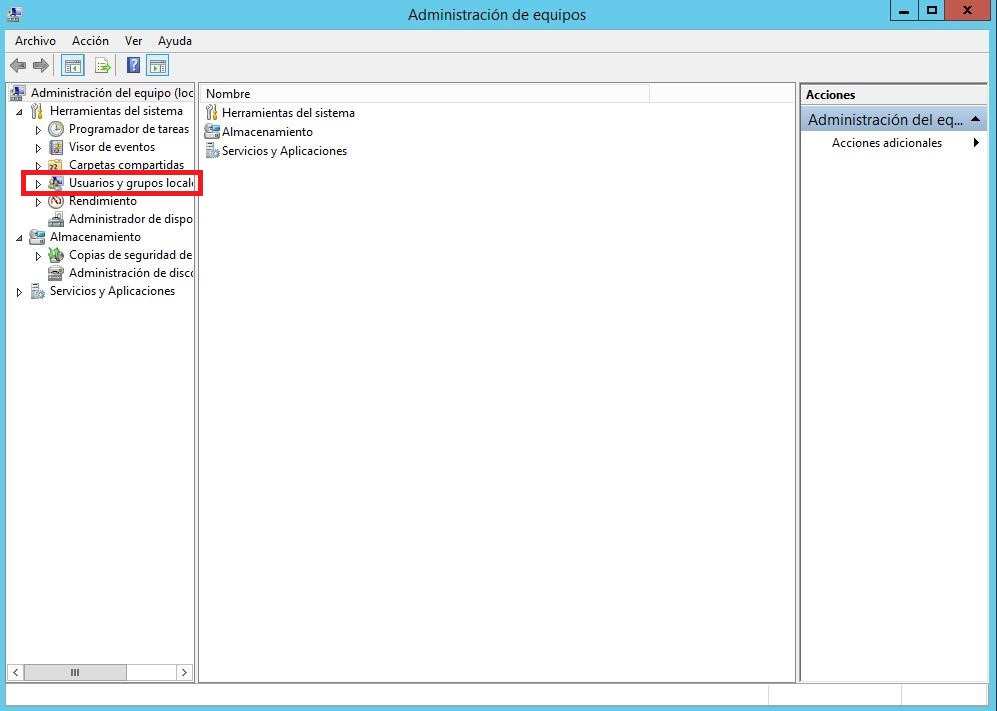
\includegraphics[width=10cm]{./Imagenes/jhordy11} 
	\end{center}
	\hfill \break
	\hfill \break
	\hfill \break
	\hfill \break
	\item Ingresamos a la carpeta de Usuarios y nos vamos a la opci\'on de equipos ORACLE.\\
	\begin{center}
	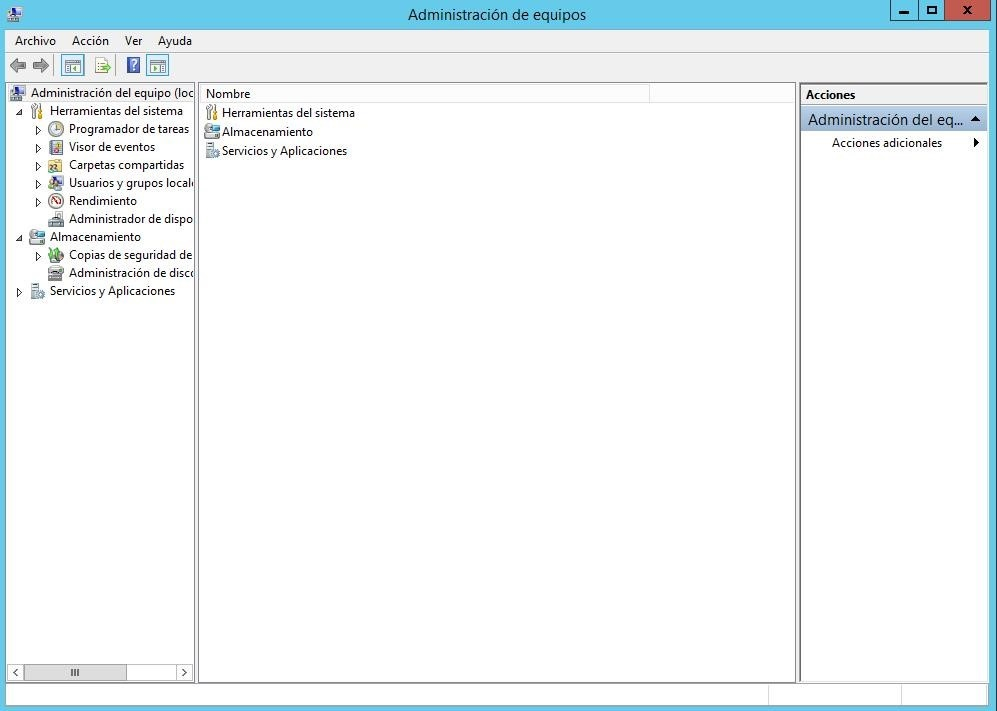
\includegraphics[width=10cm]{./Imagenes/jhordy2} 
	\end{center}
	\hfill \break
	\hfill \break
	\hfill \break
	\hfill \break
	\item Una vez realizado eso reiniciamos el servidor y al usuario ORACLE.\\
	\begin{center}
	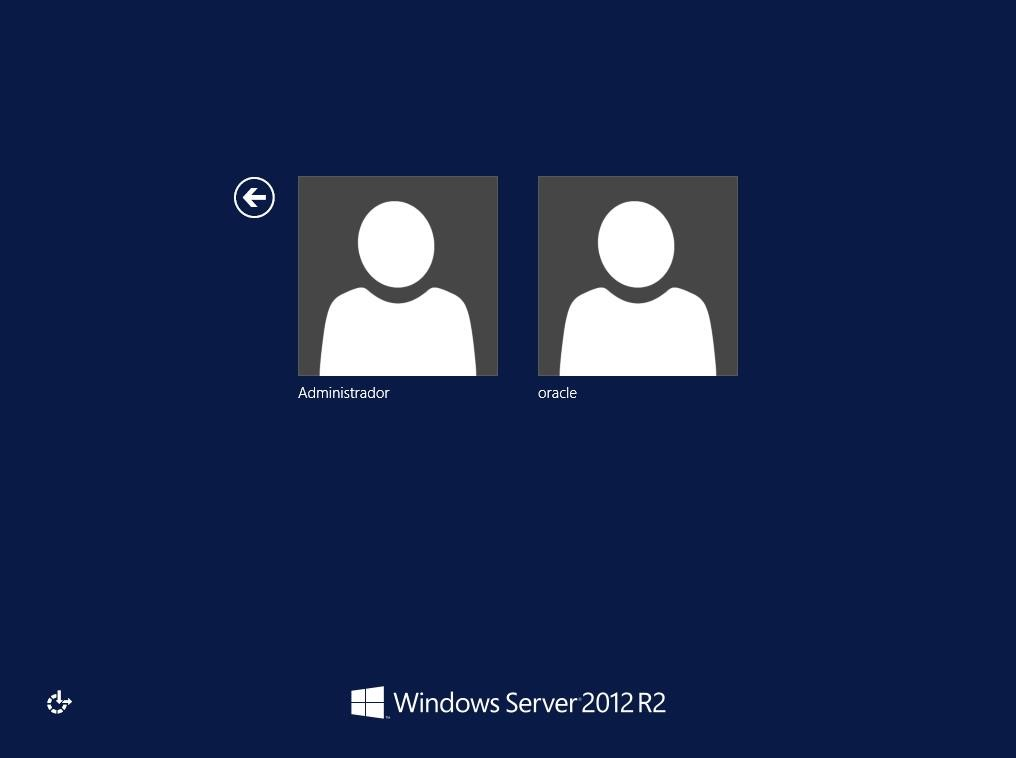
\includegraphics[width=10cm]{./Imagenes/jhordy3} 
	\end{center}
	\hfill \break
	\hfill \break
	\hfill \break
	\hfill \break
	\item Colocamos la clave de administrador que es  "UPT2018".\\
	\begin{center}
	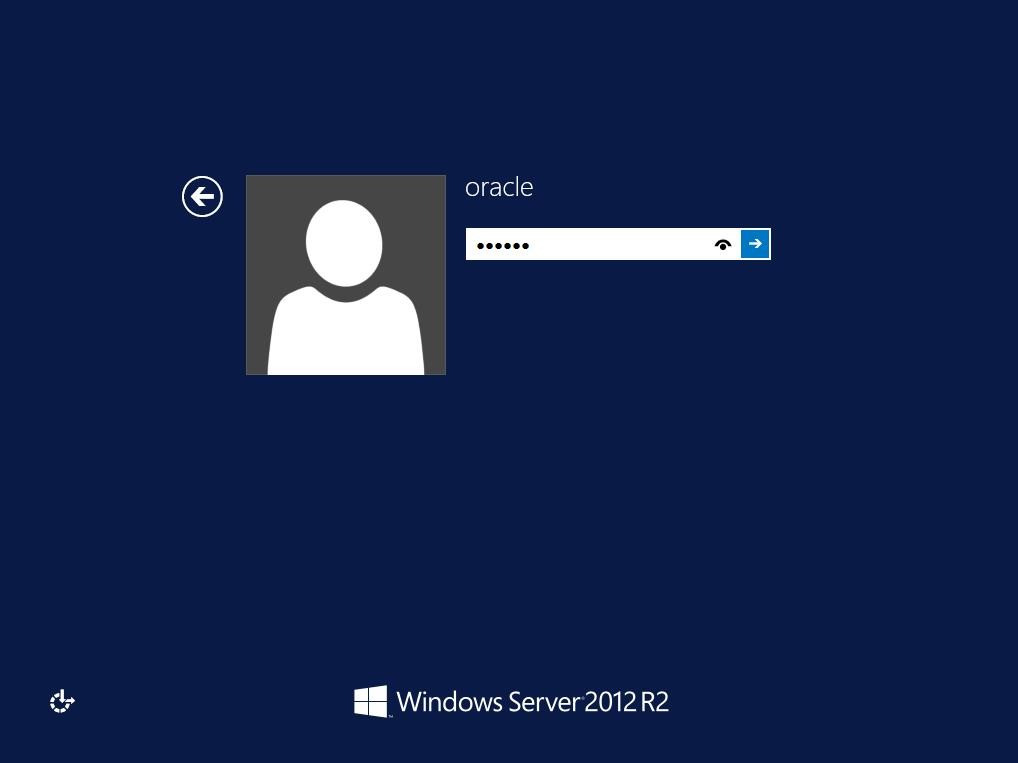
\includegraphics[width=10cm]{./Imagenes/jhordy4} 
	\end{center}
	\hfill \break
	\hfill \break
	\hfill \break
	\hfill \break
	\item Empezaremos la instalaci\'on de la base de datos ORACLE seleccionando el archivo ejecutable "setup" a setup.\\
	\begin{center}
	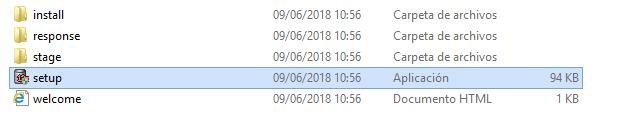
\includegraphics[width=10cm]{./Imagenes/jhordy5} 
	\end{center}
	\hfill \break
	\hfill \break
	\hfill \break
	\hfill \break
	\hfill \break
	\item Instalamos como el usuario administrador, colocando la clave de usuario.\\
	\begin{center}
	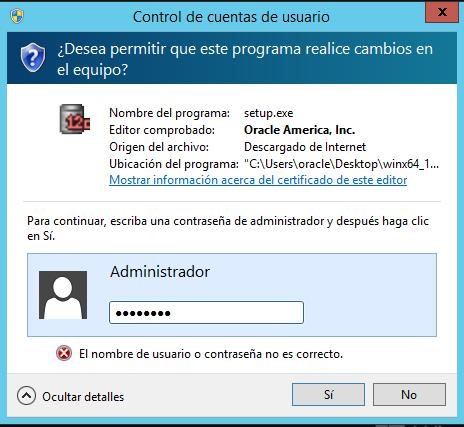
\includegraphics[width=10cm]{./Imagenes/jhordy6} 
	\end{center}
	\hfill \break
	\hfill \break
	\hfill \break
	\hfill \break
	\item Procede autom\'aticamente la instalaci\'on del ORACLE\\
	\begin{center}
	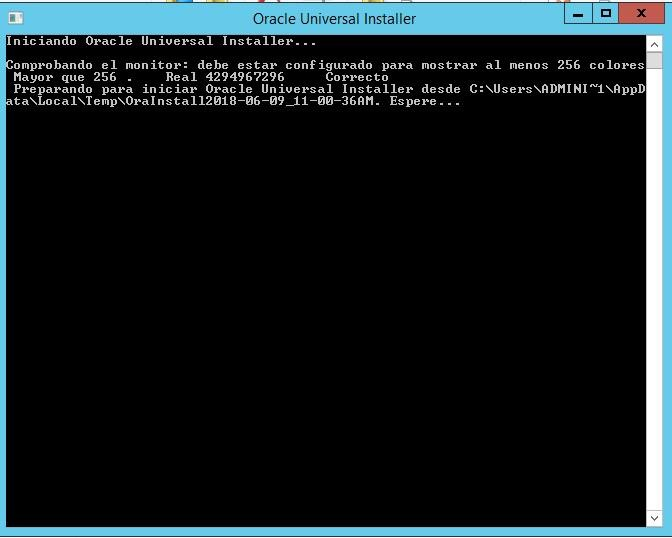
\includegraphics[width=10cm]{./Imagenes/jhordy7} 
	\end{center}
	\hfill \break
	\hfill \break
	\hfill \break
	\hfill \break
	\hfill \break
	\hfill \break
	\hfill \break
	\hfill \break
	\hfill \break
	\item Nos aparece la pantalla de configuraci\'on.\\
	\begin{center}
	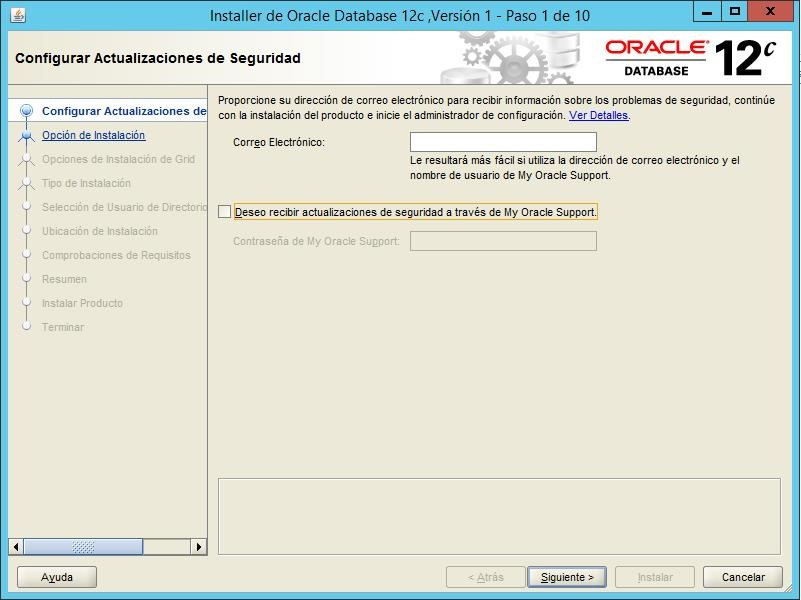
\includegraphics[width=10cm]{./Imagenes/jhordy8} 
	\end{center}
	
\end{enumerate} 
